\documentclass[a4paper,12pt]{article}
\usepackage[colorlinks=false,pdfborder=000]{hyperref}
\usepackage[top=1.2in, bottom=1.2in, left=1.2in, right=1.2in]{geometry}
\usepackage[dvips]{graphicx,color}
\usepackage{times}
\usepackage{tikz}
\usepackage{fp}
\usetikzlibrary {snakes,arrows}

%%%%%%%%%%%%%%%%%%%%%%%%%%%%%%%%%%%%%%%%%%%%%%%%%%%%%%%%%%%%%%%%%%
\def\scale{0.7}
\def\half{0.5}
\providecommand{\blockage}[4]{%
    \fill[block] (#1,#2) rectangle (#3+1,#4+1);
}
\providecommand{\drawrowcol}[2]{
    % enumerate the row and column
    \FPset{\row}{#1}
    \FPadd{\row}{\row}{-1}
    \foreach \r in {0,...,\row}
        \node at (0-\half,\r+\half) {\r} ;
    \FPset{\col}{#2}
    \FPadd{\col}{\col}{-1}
    \foreach \c in {0,...,\col}
        \node at (\c+\half,0-\half) {\c} ;
}
\providecommand{\drawgrid}[2]{
    \draw (0,0) grid (#1,#2);
    \drawrowcol{#1}{#2}
}
\providecommand{\drawtwopin}[7]{
%#1= pin1 name #2,#3=pin1 location
%#4= pin1 name #5,#6=pin2 location
%#7= color
    \node[pins,#7]  (#1) at (#2 + \half, #3 + \half) {}; % pin-1
    \node[pins,#7]  (#4) at (#5  + \half, #6 + \half) {}  % pin-2
        edge[arrow] (#1);            % arrow
    %\node[above] at (#1) {$#1$}; % label
    %\node[above] at (#4) {$#4$}; % label
}
\providecommand{\drawthreepin}[9]{
%#1= pin1 name #2,#3=pin1 location
%#4= pin1 name #5,#6=pin2 location
%#7= pin1 name #8,#9=pin3 location
    \node[pins]  (#1) at (#2 + \half, #3 + \half) {}; % pin-1
    \node[pins]  (#4) at (#5  + \half, #6 + \half) {}  % pin-2
        edge[arrow] (#1);            % arrow
    \node[pins]  (#7) at (#8  + \half, #9 + \half) {}  % pin-2
        edge[arrow] (#1);            % arrow
}
%%%%%%%%%%%%%%%%%%%%%%%%%%%%%%%%%%%%%%%%%%%%%%%%%%%%%%%%%%%%%%%%%%
\begin{document}

\begin{figure}
\centering
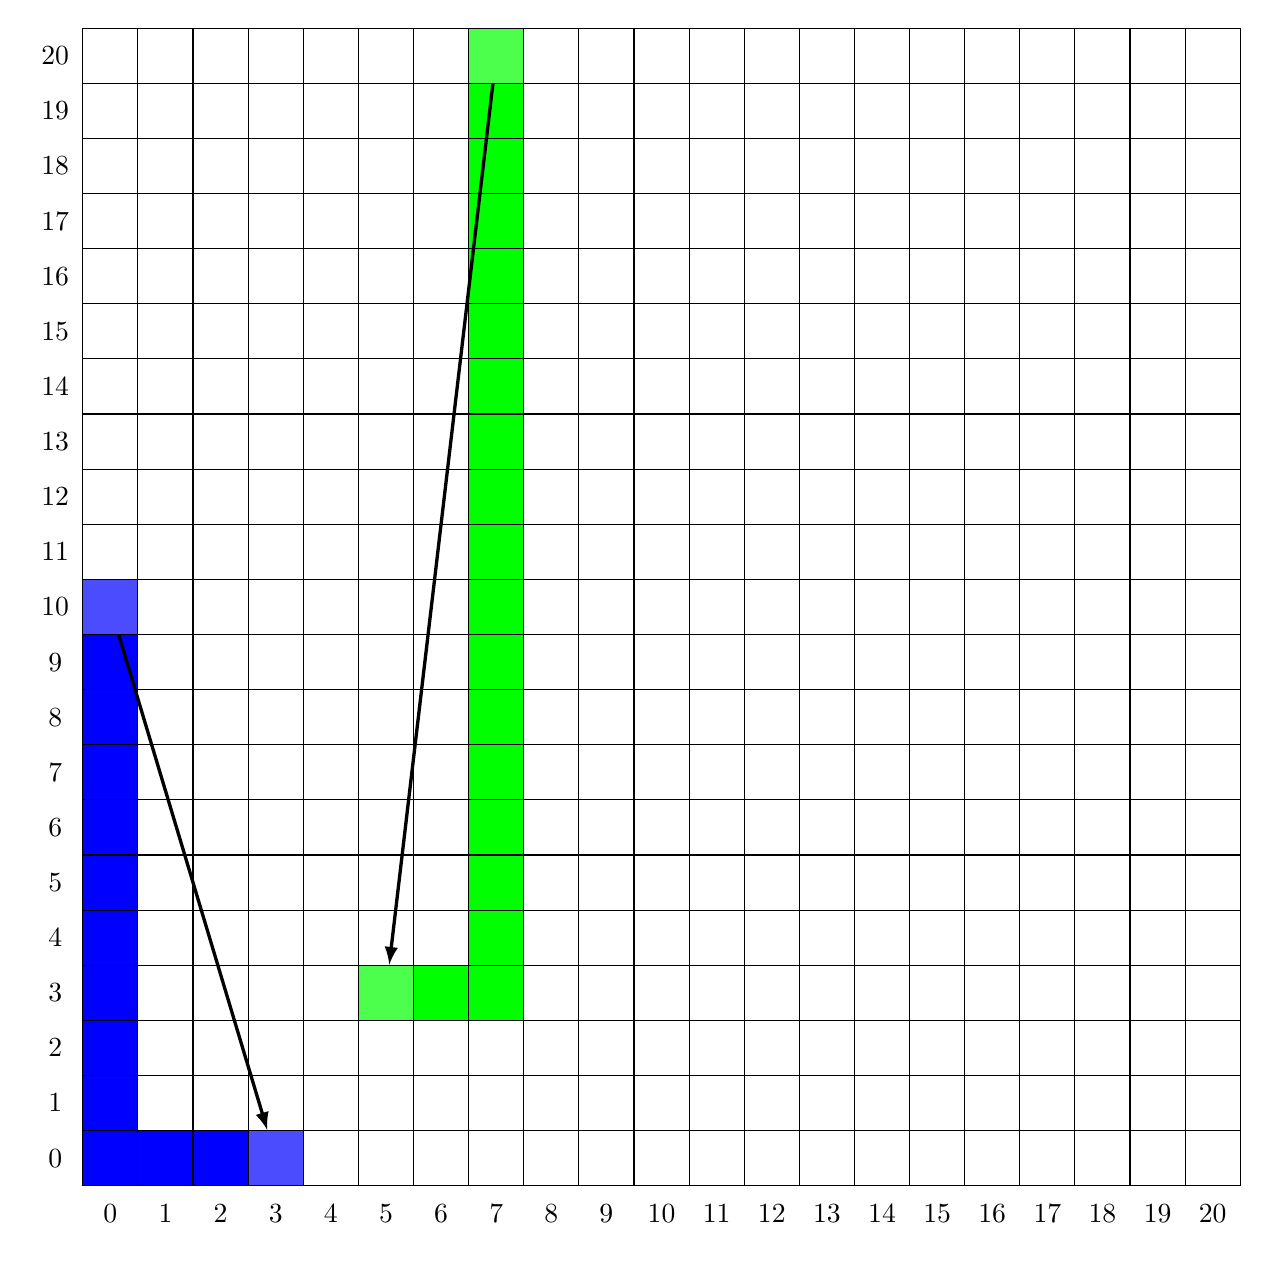
\begin{tikzpicture}[scale=\scale,
	%inner sep=1cm*\scale*\half,
	inner sep=0,
	minimum size=1cm*\scale,
	>=latex,
	pins/.style={rectangle,draw,fill=brown,font=\scriptsize},
	arrow/.style={->,very thick},
	block/.style={gray}]
	% define the row and column number
	\def \N{21}\def \M{21}
	% blockages
	% nets
	
\node[pins,blue] (net_0_0_10) at (0+\half,10+\half) {};
\node[pins,blue] (net_0_0_9) at (0+\half,9+\half) {};
\node[pins,blue] (net_0_0_8) at (0+\half,8+\half) {};
\node[pins,blue] (net_0_0_7) at (0+\half,7+\half) {};
\node[pins,blue] (net_0_0_6) at (0+\half,6+\half) {};
\node[pins,blue] (net_0_0_5) at (0+\half,5+\half) {};
\node[pins,blue] (net_0_0_4) at (0+\half,4+\half) {};
\node[pins,blue] (net_0_0_3) at (0+\half,3+\half) {};
\node[pins,blue] (net_0_0_2) at (0+\half,2+\half) {};
\node[pins,blue] (net_0_0_1) at (0+\half,1+\half) {};
\node[pins,blue] (net_0_0_0) at (0+\half,0+\half) {};
\node[pins,blue] (net_0_1_0) at (1+\half,0+\half) {};
\node[pins,blue] (net_0_2_0) at (2+\half,0+\half) {};
\node[pins,blue] (net_0_3_0) at (3+\half,0+\half) {};
\node[pins,blue] (net_0_3_0) at (3+\half,0+\half) {};
\node[pins,blue] (net_0_3_0) at (3+\half,0+\half) {};
\node[pins,blue] (net_0_3_0) at (3+\half,0+\half) {};
\node[pins,blue] (net_0_3_0) at (3+\half,0+\half) {};
\node[pins,blue] (net_0_3_0) at (3+\half,0+\half) {};
\node[pins,blue] (net_0_3_0) at (3+\half,0+\half) {};
\node[pins,blue] (net_0_3_0) at (3+\half,0+\half) {};

\node[pins,green] (net_1_7_20) at (7+\half,20+\half) {};
\node[pins,green] (net_1_7_19) at (7+\half,19+\half) {};
\node[pins,green] (net_1_7_18) at (7+\half,18+\half) {};
\node[pins,green] (net_1_7_17) at (7+\half,17+\half) {};
\node[pins,green] (net_1_7_16) at (7+\half,16+\half) {};
\node[pins,green] (net_1_7_15) at (7+\half,15+\half) {};
\node[pins,green] (net_1_7_14) at (7+\half,14+\half) {};
\node[pins,green] (net_1_7_13) at (7+\half,13+\half) {};
\node[pins,green] (net_1_7_12) at (7+\half,12+\half) {};
\node[pins,green] (net_1_7_11) at (7+\half,11+\half) {};
\node[pins,green] (net_1_7_10) at (7+\half,10+\half) {};
\node[pins,green] (net_1_7_9) at (7+\half,9+\half) {};
\node[pins,green] (net_1_7_8) at (7+\half,8+\half) {};
\node[pins,green] (net_1_7_7) at (7+\half,7+\half) {};
\node[pins,green] (net_1_7_6) at (7+\half,6+\half) {};
\node[pins,green] (net_1_7_5) at (7+\half,5+\half) {};
\node[pins,green] (net_1_7_4) at (7+\half,4+\half) {};
\node[pins,green] (net_1_7_3) at (7+\half,3+\half) {};
\node[pins,green] (net_1_6_3) at (6+\half,3+\half) {};
\node[pins,green] (net_1_5_3) at (5+\half,3+\half) {};
\node[pins,green] (net_1_5_3) at (5+\half,3+\half) {};

\drawtwopin{Dlt01}{3}{0}{Sample}{0}{10}{blue!70}
\drawtwopin{Dlt01}{5}{3}{B1}{7}{20}{green!70}
\drawgrid{\N}{\M}
	\end{tikzpicture}
      \end{figure}
      \end{document}
